\subsection{Trajectory Comparison in Three-Dimensional Forests}
We further evaluate the frozen planners in a forest environment and visualize their executed trajectories at two obstacle densities, following the scene-level comparison used in YOPO~\cite{lu2024yopo}. Eight paired seeds generate 40 and 80 tree centers within a $200\times160$ m region, corresponding to $1/800$ and $1/400$ tree/m$^2$. Each tree consists of a cylindrical trunk with radius $0.8$--$1.4$ m and height $24$--$36$ m, together with a spherical crown of radius $4$--$6$ m. Twelve low spherical bushes are shared by each pair. The dense map retains every sparse-map obstacle and adds 40 trees. All five methods start at $(0,0,20)$ m with an airspeed of $15.5$ m/s and approach the target at $(250,0,20)$ m. The nominal execution model, planner settings and network weights remain unchanged. This experiment comprises 80 episodes on 16 additional maps.

Figure~\ref{fig:forestcomparison} shows the first seed, fixed for both panels before execution. The height-colored surfaces represent the collision geometry, and each curve connects recorded flight states. All methods complete the eight sparse-forest tasks. In the dense forests, Learned completes seven tasks and terminates at an inflated obstacle margin in one; Cost, Diverse, No-geometry and Full each complete all eight. This termination appears in the displayed dense scene, where Learned initially follows a different route and ends before reaching the goal region. Cost and Full select identical trajectories in both displayed scenes. These examples illustrate how continuation-query ordering changes the executed route, while the broader forest comparison shows little separation in completion across the tested methods.

\begin{figure*}[!t]
\centering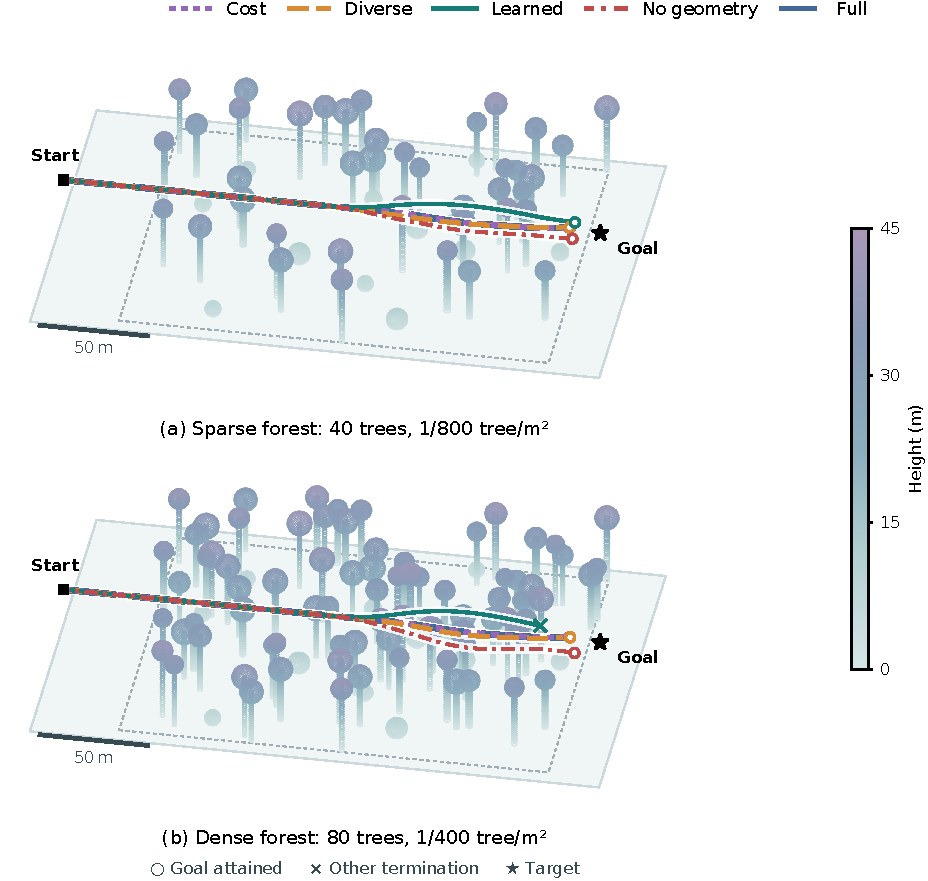
\includegraphics[width=.94\textwidth]{figures/forest_comparison.pdf}
\caption{Nominal closed-loop trajectories in paired sparse and dense forests (seed 601000). Height-colored samples visualize the analytic obstacle surfaces; curves show recorded execution states. The dense map retains the 40 sparse-map trees and adds 40, while 12 bushes remain common. Circles mark goal attainment and the cross marks termination at an inflated obstacle margin. Cost and Full coincide in this pair. The dashed ground rectangle denotes the region used to calculate tree-center density.}
\label{fig:forestcomparison}
\end{figure*}
